\documentclass[2pt,-letter paper]{article}
\usepackage{graphicx} % Required for inserting images
\usepackage{siunitx}
\usepackage{setspace}
\usepackage{gensymb}
\usepackage{xcolor}
\usepackage{caption}
%\usepackage{subcaption}
\doublespacing
\singlespacing
\usepackage[none]{hyphenat}
\usepackage{amssymb}
\usepackage{relsize}
\usepackage[cmex10]{amsmath}
\usepackage{mathtools}
\usepackage{amsmath}
\usepackage{commath}
\usepackage{amsthm}
\interdisplaylinepenalty=2500
%\savesymbol{iint}
\usepackage{txfonts}
%\restoresymbol{TXF}{iint}
\usepackage{wasysym}
\usepackage{amsthm}
\usepackage{mathrsfs}
\usepackage{txfonts}
\let\vec\mathbf{}
\usepackage{stfloats}
\usepackage{float}
\usepackage{cite}
\usepackage{cases}
\usepackage{subfig}
%\usepackage{xtab}
\usepackage{longtable}
\usepackage{multirow}
%\usepackage{algorithm}
\usepackage{amssymb}
%\usepackage{algpseudocode}
\usepackage{enumitem}
\usepackage{mathtools}
%\usepackage{eenrc}
%\usepackage[framemethod=tikz]{mdframed}
\usepackage{listings}
%\usepackage{listings}
\usepackage[latin1]{inputenc}
%%\usepackage{color}{   
%%\usepackage{lscape}
\usepackage{textcomp}
\usepackage{titling}
\usepackage{hyperref}
%\usepackage{fulbigskip}   
\usepackage{tikz}
\usepackage{graphicx}
\lstset{
  frame=single,
  breaklines=true
}
\let\vec\mathbf{}
\usepackage{enumitem}
\usepackage{graphicx}
\usepackage{siunitx}
\let\vec\mathbf{}
\usepackage{enumitem}
\usepackage{graphicx}
\usepackage{enumitem}
\usepackage{tfrupee}
\usepackage{amsmath}
\usepackage{amssymb}
\usepackage{mwe} % for blindtext and example-image-a in example
\usepackage{wrapfig}
\graphicspath{{figs/}}
\providecommand{\mydet}[1]{\ensuremath{\begin{vmatrix}#1\end{vmatrix}}}
\providecommand{\myvec}[1]{\ensuremath{\begin{bmatrix}#1\end{bmatrix}}}
\providecommand{\cbrak}[1]{\ensuremath{\left\{#1\right\}}}
\providecommand{\brak}[1]{\ensuremath{\left(#1\right)}}

  

\title{MATHEMATICS}
\author{Lakshmipriya Patibandla}
\date{\today}

\begin{document}

\maketitle
\begin{enumerate}
\section{Discrete}

\item The HCF of two numbers $a$ and $b$ is $5$ and their LCM is $200 $. Find the product $ab$.

\item Find the HCF of $612$ and $1314$ using prime factorisation.

\item Show that any positive odd integer is of the form $6m + 1$ or $6m + 3$ or $6m + 5$, where $m$ is some integer.

\item Prove that ${\sqrt 5}$ is an irrational number.

\item Prove that $\brak{5 - 3{\sqrt 2}}$ is an irrational number, given that ${\sqrt2}$ is irrational number.

\item Find the sum of all the two digit numbers which leave the remainder $2$ when divided by $5$.

\item If in an A.P ., $a=15$,$d=-3$ and $a_n=0$, then find the value of $n$.

\item If ${S_n}$, the sum of the first ${n}$ terms of an A.P. is given by ${S_n = 2n^2 + n}$,then find its $n^{th}$ term. 

\item If the $17^{th}$ term of an A.P. exceeds its $10^{th}$ term by $7$, find the common difference.

\item If the sum of the first $p$ terms of an A.P. is $q$ and the sum of the first $q$ terms is $p$; then show that the sum of the first $\brak{p + q}$ terms is $\cbrak {-\brak {p + q}}$.

\item Write the common difference of the A.P.${\sqrt3} , {\sqrt12} , {\sqrt27} , {\sqrt48}$ , ... 

\item In an A.P., the $n^{th}$ term is ${\frac{1}{m}}$ and the $m^{th}$ term is $\frac{1}{n}$. Find \begin{enumerate}
     \item  $\brak{mn}^{th}$term  ,
     \item sum of first $\brak{mn}$ terms.
\end{enumerate}

\section{Algebra}

\item Find all the zeroes of the polynomial $x^4 + x^3- 14x^2 -2x + 24$, if two of its zeroes are $\sqrt2$ and $-\sqrt 2$ .

\item Apply division algorithm to check if $g\brak{x} = x^2 - 3x + 2$ is a factor of the polynomial $f\brak{x} = x^4 - 2x^3 - x + 2$.


\item A train travels $360 km$ at a uniform speed. If the speed had been $5 km/hr$ more, it would have taken $1 hr$ less for the same journey. Find the speed of the train.

\item Find the value of $k$ for which $x = 2$ is a solution of the equation
  $kx^2 + 2x - 3 = 0$.
  
\item Find the value/s of $k$ for which the quadratic equation $3x^{2} + kx + 3 = 0$
has real and equal roots.


\item Solve for $x$ :
\begin{align*}
    {\frac {1}{a+b+x}} = {\frac{1}{a}} + {\frac{1}{b}} + {\frac{1}{x}};  {a\neq b \neq 0},{x \neq 0},{x \neq -(a+b)}
\end{align*}

\item If $\sin{x} + \cos{y}= 1$ ; $x=30\degree$  and  $y$ is an acute angle, find the value of $y$ .

\item Find the value of $\cos {48\degree} - \sin {42\degree}$.

\item Prove that :
\begin{align*}
   {\frac{\tan\theta}{1-\tan\theta}} - {\frac{\cot\theta}{1-\cot\theta}}={\frac{\cos\theta+ \sin\theta}{\cos\theta-\sin\theta}}
\end{align*} 

\item If ${\cos\theta + \sin\theta} = {\sqrt 2}{\cos\theta}$, show that ${\cos\theta - \sin\theta} = {\sqrt 2}{\sin\theta}$.

\item Prove that :
\begin{align*}
    {\frac{(1+\cot\theta+\tan\theta)(\sin\theta-\cos\theta)}{(\sec^3\theta-\csc^3\theta)}} = \sin^2\theta \cos^2\theta
\end{align*}

\item Evaluate :
\begin{align*}
    {\frac{\csc^2(90\degree - \theta)-\tan^2\theta)}{2(\cos^2 37\degree + \cos^2 53\degree)}} - {\frac{2\tan^2 30\degree \sec^2 37\degree \cdot \sin^2 53\degree}{\csc^2 63\degree - \tan^2 27\degree}} 
\end{align*}

\section{Matrices}

\item For what value of $k$, does the system of linear equations\\
\begin{align*}
   2x + 3y = 7\\
 \brak{k - 1} x + \brak{k + 2} y = 3k
\end{align*}
have an infinite number of solutions ?

\item A part of monthly hostel charges in a college hostel are fixed and the remaining depends on the number of days one has taken food in the mess. When a student $A$ takes food for $25$ days, he has to pay {\rupee $4,500$}, whereas a student $B$ who takes food for $30$ days, has to pay {\rupee $5,200$}. Find the fixed charges per month and the cost of food per day.

\section{Vectors}

\item Find the value of '$a$' so that the point $\brak{3, a}$ lies on the line represented
by $2 x - 3 y = 5$.

\item The mid-point of the line segment joining $A\brak{2a, 4}$ and $B\brak{-2, 3b}$ is $\brak{1, 2a + 1}$. Find the values of $a$ and $b$.

\item Point P divides the line segment joining the points $A\brak{2, 1}$ and $B\brak{5, -8}$ such that $\frac{AP}{AB}$ = $\frac{1}{3}$.If $P$ lies on the line $2x - y + k = 0$, find the value of $k$.

\item For what value of $p$, are the points $\brak{2, 1}$, $\brak{p,- 1}$ and $\brak{- 1, 3}$ collinear ?

\item Find the coordinates of a point $A$, where $AB$ is a diameter of the circle with centre $\brak{3, -1}$ and the point $B$ is $\brak{2, 6}$.

\item Find the values of $x$ for which the distance between the points $A\brak{x, 2}$ and $B\brak{9, 8}$ is $10$ units.

\item The mid-point of the line segment joining $A\brak{2a, 4}$ and $B\brak{-2, 3b}$ is $\brak{1, 2a + 1}$. Find the values of $a$ and $b$.

\section{Construction}

\item Prove that tangents drawn at the ends of a diameter of a circle are parallel.

\item The area of two similar triangles are $25 sq. cm$ and $121 sq. cm$. Find the
ratio of their corresponding sides.

\item In \figref{fig:Fig-1}, $E$ is a point on $CB$ produced of an isosceles ${\triangle ABC}$, with side $AB$ = $AC$. If ${AD \perp  BC }$ and ${ EF \perp AC}$, prove that ${\triangle ABD{ \sim }\triangle ECF}$.
 \begin{figure}[H]
    \centering
    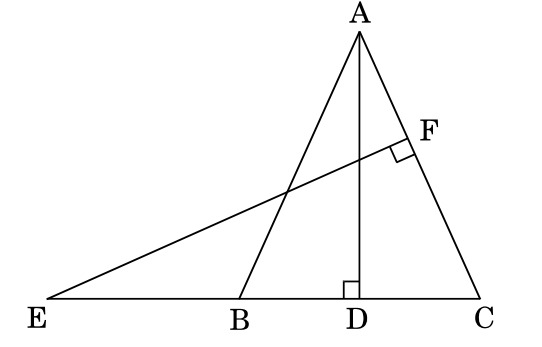
\includegraphics[width=\columnwidth]{figures/Figure_1.png}
    \caption{Triangle}
    \label{fig:Fig-1}
\end{figure}

\item Prove that the parallelogram circumscribing a circle is a rhombus.

\item In a triangle, if the square of one side is equal to the sum of the squares of the other two sides, then prove that the angle opposite to the first side is a right angle.

\item In two concentric circles, prove that all chords of the outer circle which touch the inner circle, are of equal length.

\item Construct an isosceles triangle whose base is $8 cm$ and altitude $4 cm$ and then another triangle whose sides are $\frac{3}{4}$ times the corresponding sides of the isosceles triangle.

\item Construct a right triangle in which sides (other than the hypotenuse) are $8 cm$ and $6 cm$. Then construct another triangle whose sides are $\frac{5}{3}$ times the corresponding sides of the right triangle.

\item Construct a pair of tangents to a circle of radius $4 cm$ which are inclined to each other at an angle of $60\degree$.

\item In ${\triangle ABC}$, ${\angle B} = {90\degree}$ and $D$ is the mid-point of $BC$. Prove that ${AC}^2 = {AD}^2 + 3{CD}^2$.

\item Prove that in a right triangle, the square of the hypotenuse is equal to the sum of the squares of the other two sides.

\section{Trigonometry}

\item A boy standing on a horizontal plane finds a bird flying at a distance of $100 m$ from him at an elevation of $30\degree$. A girl standing on the roof of a $20 m$ high building, finds the elevation of the same bird to be $45\degree$. The boy and the girl are on the opposite sides of the bird. Find the distance of the bird from the girl. (Given ${\sqrt 2}= 1.414$)

\item The angle of elevation of an aeroplane from a point $A$ on the ground is $60\degree$. After a flight of $30 $seconds , the angle of elevation changes to $30\degree$. If the plane is flying at a constant height of $3600\sqrt 3 $ metres, find the speed of the aeroplane.

\section{Geometry}

\item In \figref{fig:Fig-2}, three sectors of a circle of radius $7cm$, making angles of $60\degree$,
$80\degree$ and $40\degree$ at the centre are shaded. Find the the area of the shaded region.
\begin{figure}[H]
    \centering
    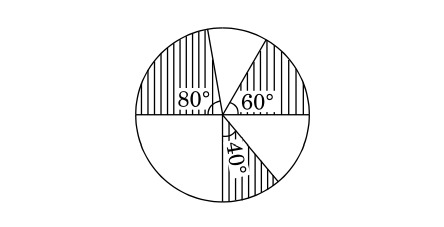
\includegraphics[width=\columnwidth]{figures/Figure_2.png}
    \caption{Circle}
    \label{fig:Fig-2}
\end{figure}

\item A juice seller was serving his customers using glasses as shown in \figref{fig:Fig-3} . The inner diameter of the cylindrical glass was $5 cm$ but bottom of the glass had a hemispherical raised portion which reduced the capacity of the glass. If the height of a glass was $10 cm$, find the apparent and actual capacity of the glass. (Use $\pi = 3.14$ )
\begin{figure}[H]
    \centering
    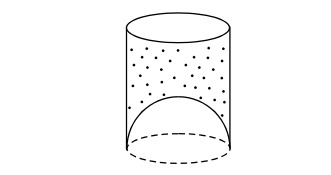
\includegraphics[width=\columnwidth]{figures/Figure_3.png}
    \caption{Hemisphere}
    
    \label{fig:Fig-3}
\end{figure}

\item A girl empties a cylindrical bucket full of sand, of base radius $18 cm$ and height $32 cm$ on the floor to form a conical heap of sand. If the height of this conical heap is $24 cm$, then find its slant height correct to one place of decimal.

\item An open metallic bucket is in the shape of a frustum of a cone. If the diameters of the two circular ends of the bucket are $45 cm$ and $25 cm$ and the vertical height of the bucket is $24 cm$, find the area of the metallic sheet used to make the bucket. Also find the volume of the water it can 
hold. (Use $\pi =\frac{22}{7}$)

\section{Probability}

\item A child has a die whose $6$ faces show the letters given below :
\begin{align*}
    { \framebox {A} \hspace{1cm}} {\framebox {B} \hspace{1cm}} {\framebox {C}\hspace{1cm}} {\framebox {A}\hspace{1cm}} {\framebox {A}\hspace{1cm}} {\framebox {B}}
\end{align*}

\item Cards marked with numbers $5$ to $50$ (one number on one card) are placed in a box and mixed thoroughly. One card is drawn at random from the box. Find the probability that the number on the card taken out is \begin{enumerate}
    \item a prime number less than $10$,  
    \item a number which is a perfect square.
\end{enumerate}

\item Find the probability that a number selected at random from the numbers $3, 4, 4, 4, 5, 5, 6, 6, 6, 7$ will be their mean.


\end{enumerate}
\end{document}
